\appendix

\section{Hyperparameter Configuration}
\label{app:hyperparams}

Table~\ref{tab:hyperparams} lists the full hyperparameter configuration used for PCGT across all 14 datasets. Most medium-scale experiments use hidden dimension $d=64$; Deezer uses $d=96$ due to its larger feature space (31K features). All experiments use a single PCGT attention layer ($L_\text{pcgt}=1$), $M=4$ learned seeds per partition, and the METIS partitioning algorithm. The large-scale experiments (ogbn-arxiv, pokec, Amazon2M) use $d=256$ and mini-batch training with batch size 100K.

\begin{table*}[t]
\centering
\small
\resizebox{\textwidth}{!}{%
\begin{tabular}{l|ccccccccccc}
\toprule
\textbf{Dataset} & $d$ & \textbf{$K$} & $L_\text{gcn}$ & \textbf{lr} & \textbf{WD} & \textbf{Dropout} & $\lambda_\text{gw}$ & \textbf{Attn Drop} & \textbf{Attn WD} & \textbf{Epochs} & \textbf{Runs} \\
\midrule
Cora         & 64  & 10  & 2 & 0.01  & 5e-4  & 0.4 & 0.8 & 0.2 & 1e-3 & 500  & 10 \\
CiteSeer     & 64  & 20  & 2 & 0.01  & 0.01  & 0.5 & 0.7 & 0.3 & 0.01 & 500  & 10 \\
PubMed       & 64  & 50  & 2 & 0.01  & 5e-4  & 0.5 & 0.8 & 0.3 & 0.01 & 500  & 10 \\
Chameleon    & 64  & 10  & 2 & 0.01  & 1e-3  & 0.5 & 0.8 & 0.3 & 0.01 & 500  & 10 \\
Squirrel     & 64  & 10  & 4 & 0.01  & 5e-4  & 0.5 & 0.8 & 0.3 & 0.01 & 500  & 10 \\
Film         & 64  & 5   & 2 & 0.05  & 5e-4  & 0.5 & 0.5 & 0.3 & 0.01 & 500  & 10 \\
Deezer       & 96  & 20  & 2 & 0.01  & 5e-5  & 0.4 & 0.5 & 0.4 & 5e-5 & 500  & 5 \\
Co-CS        & 64  & 15  & 4 & 0.01  & 5e-4  & 0.5 & 0.8 & 0.2 & 1e-3 & 500  & 10 \\
Co-Phys.     & 64  & 20  & 4 & 0.01  & 5e-4  & 0.5 & 0.8 & 0.2 & 1e-3 & 500  & 10 \\
Am-Comp.     & 64  & 10  & 4 & 0.01  & 5e-4  & 0.5 & 0.8 & 0.2 & 1e-3 & 500  & 10 \\
Am-Photo     & 64  & 10  & 4 & 0.01  & 5e-4  & 0.5 & 0.8 & 0.2 & 1e-3 & 500  & 10 \\
\midrule
ogbn-arxiv   & 256 & 256 & 3 & 0.001 & 0     & 0.5 & 0.5 & 0.5 & 0    & 1000 & 10 \\
pokec        & 64  & 500 & 2 & 0.01  & 0     & 0   & 0.5 & 0   & 0    & 1000 & 3 \\
Amazon2M     & 256 & 1000 & 3 & 0.01 & 0     & 0   & 0.5 & 0   & 0    & 1000 & 3 \\
\bottomrule
\end{tabular}
}% end resizebox
\caption{PCGT hyperparameters for all datasets. $d$: hidden dimension; $K$: number of METIS partitions; $L_\text{gcn}$: GCN backbone layers; WD: weight decay (GCN branch); Attn Drop/WD: dropout and weight decay for the PCGT attention parameters. All experiments use $M=4$ seeds, Adam optimizer, and early stopping with patience 200.}
\label{tab:hyperparams}
\end{table*}

\section{Complexity Derivation}
\label{app:complexity}

We derive the per-layer computational complexity of PCGT. Let $N$ be the number of nodes, $K$ the number of partitions, $M$ the number of seeds per partition, $d$ the hidden dimension, and $|E|$ the number of edges.

\textbf{Local attention.}~~For a balanced partition, each group contains approximately $N/K$ nodes. Standard self-attention within one partition costs $O((N/K)^2 \cdot d) = O(N^2 d / K^2)$. Summing over all $K$ partitions:
\begin{equation}
C_\text{local} = K \cdot O\!\left(\frac{N^2 d}{K^2}\right) = O\!\left(\frac{N^2 d}{K}\right)
\label{eq:local_cost}
\end{equation}
This achieves a $K$-fold reduction over full $O(N^2 d)$ attention while retaining exact (non-approximated) attention within each partition.

\textbf{Seed pooling.}~~For each of the $K$ partitions, the $M$ seed queries attend over $N/K$ keys to produce $M$ representative vectors. This costs $O(M \cdot (N/K) \cdot d)$ per partition, and summing over $K$ partitions:
\begin{equation}
C_\text{pool} = K \cdot O\!\left(\frac{MNd}{K}\right) = O(MNd)
\label{eq:pool_cost}
\end{equation}

\textbf{Global cross-attention.}~~Each of the $N$ node queries attends over $KM$ representative keys, costing:
\begin{equation}
C_\text{global} = O(N \cdot KM \cdot d)
\label{eq:global_cost}
\end{equation}

\textbf{GCN branch.}~~The multi-layer GCN costs $O(|E| \cdot d)$ per layer, which is standard.

\textbf{Total PCGT layer cost:}
\begin{equation}
C_\text{PCGT} = \underbrace{O\!\left(\frac{N^2 d}{K}\right)}_{\text{local attn}} + \underbrace{O(NMKd)}_{\text{global attn + pool}} + \underbrace{O(|E|d)}_{\text{GCN}} 
\label{eq:total_cost}
\end{equation}
Dropping the constant $d$ factor and noting $C_\text{pool} \subseteq C_\text{global}$, we write the complexity as $O(N^2/K + NMK + |E|)$.

\textbf{Practical regime.}~~For typical settings ($N$=10K, $K$=10, $M$=4): $N^2/K = 10$M and $NMK = 400$K, giving $\sim$10.4M operations vs.\ 100M for full $O(N^2)$ attention---a $\sim$10$\times$ reduction. For ogbn-arxiv ($N$=169K, $K$=256, $M$=4): $N^2/K \approx 112$M and $NMK \approx 173$M, totaling $\sim$285M vs.\ 28.6B for full attention---a $\sim$100$\times$ reduction.

\section{Reproducibility Details}
\label{app:reproducibility}

\textbf{Hardware.}~~All experiments were conducted on a single NVIDIA H100 80GB GPU with an AMD EPYC 7763 CPU and 256GB RAM, running CUDA 12.4.

\textbf{Software.}~~PyTorch 2.6.0, PyTorch Geometric 2.7.0, OGB 1.3.6, pymetis 2025.2, Python 3.12.

\textbf{Training protocol.}~~We use early stopping based on validation accuracy with a patience of 200 epochs. The test accuracy at the epoch with the highest validation accuracy is reported (``Highest Test''). All random seeds start from 123 and increment by 1 per run. METIS partitioning is computed once as a preprocessing step and reused across all epochs and runs.

\textbf{Partition preprocessing.}~~METIS partitioning takes $<$1 second for all medium-scale datasets and $\sim$3 seconds for ogbn-arxiv. This is a one-time cost that is amortized over training.

\section{Runtime Comparison}
\label{app:runtime}

Figure~\ref{fig:runtime} visualizes the per-epoch training time from Table~\ref{tab:runtime} on a log scale. For most datasets, PCGT's overhead is 1.7--3.5$\times$ over SGFormer. The PubMed outlier (11.2$\times$) is due to its large $K$=50, which still results in a tractable 61\,ms/epoch on H100.

\begin{figure}[t]
\centering
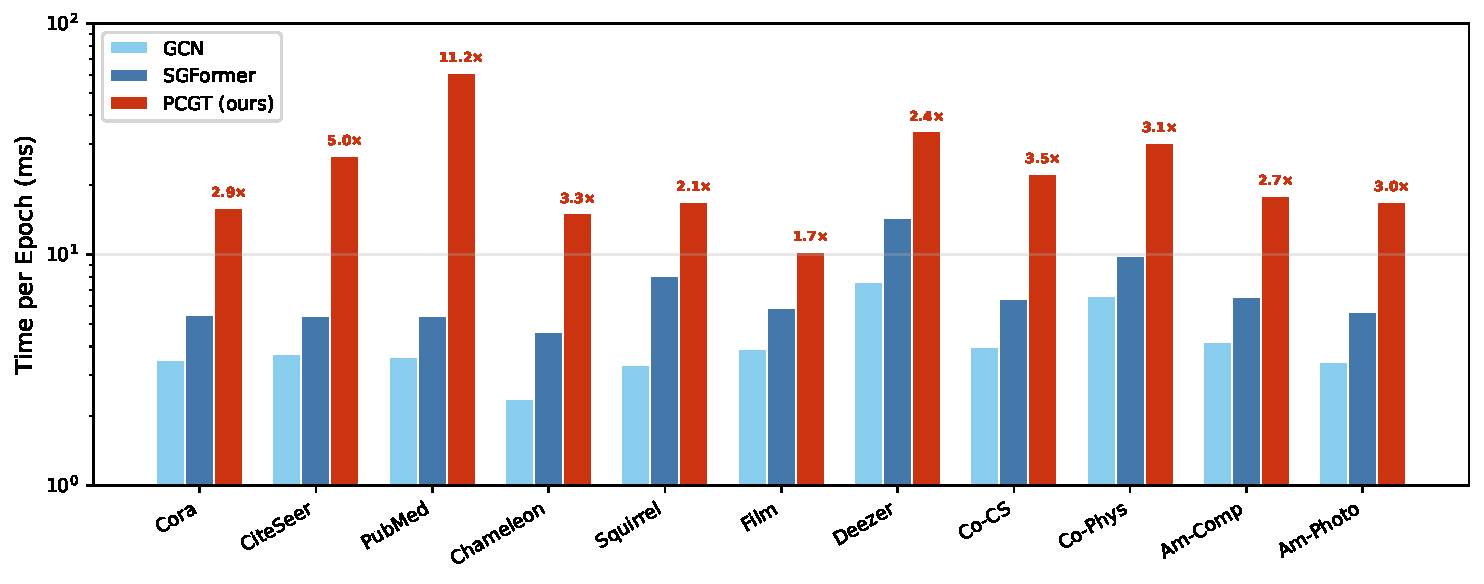
\includegraphics[width=\columnwidth]{figures/runtime_comparison.pdf}
\caption{Per-epoch training time (ms, log scale) on H100. Numbers above PCGT bars show the PCGT/SGFormer overhead ratio. The overhead is moderate and predictable, scaling with $K$ and $N$.}
\label{fig:runtime}
\end{figure}

\section{Sensitivity to Number of Seeds $M$}
\label{app:m_ablation}

Table~\ref{tab:m_ablation} varies the number of learned seeds per partition $M \in \{2, 4, 8\}$ while keeping all other hyperparameters fixed. Performance is stable: the maximum spread is 0.26 points on Cora, 0.94 on Chameleon, and 1.25 on Squirrel---all within one standard deviation. We use $M=4$ throughout.

\begin{table}[t]
\centering
\small
\begin{tabular}{c|ccc}
\toprule
$M$ & \textbf{Cora} & \textbf{Cham.} & \textbf{Sqrl.} \\
\midrule
2 & 84.46{\scriptsize$\pm$0.59} & 47.53{\scriptsize$\pm$2.53} & 46.52{\scriptsize$\pm$1.87} \\
4 & 84.52{\scriptsize$\pm$0.48} & 48.18{\scriptsize$\pm$2.94} & 47.01{\scriptsize$\pm$0.93} \\
8 & 84.26{\scriptsize$\pm$0.84} & 48.47{\scriptsize$\pm$3.04} & 45.76{\scriptsize$\pm$1.11} \\
\bottomrule
\end{tabular}
\caption{Effect of number of seeds $M$ per partition (5 runs each). Differences are within noise; $M=4$ is used throughout.}
\label{tab:m_ablation}
\end{table}

\section{Convergence Behavior}
\label{app:convergence}

Figure~\ref{fig:convergence} shows validation accuracy curves (mean $\pm$ std over 3 seeds) on three datasets spanning homophilic (Cora, PubMed) and heterophilic (Chameleon) regimes. The purpose is to compare \emph{convergence speed}, not final accuracy (which is reported in Table~\ref{tab:main} over 10 runs). Both methods reach plateau validation within similar epoch ranges and trigger early stopping at similar points, confirming that the per-epoch overhead in Table~\ref{tab:runtime} directly translates to total training overhead with no convergence penalty.

\begin{figure}[t]
\centering
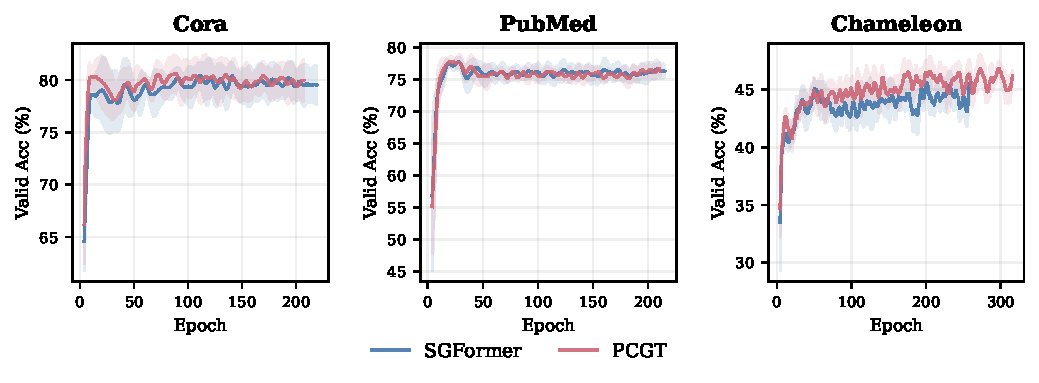
\includegraphics[width=\columnwidth]{figures/convergence.pdf}
\caption{Validation accuracy vs.\ epoch (mean $\pm$ std, 3 seeds) on Cora, PubMed, and Chameleon. Both methods converge at similar speeds. The figure illustrates convergence behavior; final accuracy comparisons use 10-run means (Table~\ref{tab:main}).}
\label{fig:convergence}
\end{figure}

\section{Statistical Significance}
\label{app:significance}

For the four additional datasets (Table~\ref{tab:new_datasets}) where we run both PCGT and SGFormer under identical code, splits, and 10 random seeds, Table~\ref{tab:pvalues} reports Welch's $t$-test $p$-values.  Coauthor-Physics shows a statistically significant improvement ($p = 0.004$), Amazon-Computers is marginally significant ($p = 0.051$), and the remaining two datasets show gains that are within noise.  For the seven Table~\ref{tab:main} datasets, SGFormer baselines are taken from the published numbers of \citet{wu2023sgformer} and per-run data is unavailable, so $t$-tests cannot be computed.

\begin{table}[t]
\centering
\small
\begin{tabular}{l|cc|cc}
\toprule
\textbf{Dataset} & \textbf{PCGT} & \textbf{SGFormer} & $\Delta$ & $p$ \\
\midrule
Co-CS        & 95.06{\scriptsize$\pm$0.32} & 94.94{\scriptsize$\pm$0.46} & +0.12 & 0.240 \\
Co-Physics   & 96.83{\scriptsize$\pm$0.16} & 96.62{\scriptsize$\pm$0.14} & +0.20 & 0.004** \\
Am-Computers & 88.80{\scriptsize$\pm$0.64} & 87.50{\scriptsize$\pm$1.88} & +1.30 & 0.051 \\
Am-Photo     & 95.27{\scriptsize$\pm$0.38} & 95.20{\scriptsize$\pm$1.12} & +0.07 & 0.822 \\
\bottomrule
\end{tabular}
\caption{Welch's $t$-test ($n=10$ runs). $**$: $p < 0.01$.  On homophilic datasets where both methods already perform well, differences are small.  PCGT's largest gains are on heterophilic benchmarks (Table~\ref{tab:main}), where published baselines preclude per-run tests.}
\label{tab:pvalues}
\end{table}

\section{Learned Self-Connection Weight $\beta$}
\label{app:beta}
\label{app:beta_prop}

\begin{proposition}[Sign of optimal $\beta$]
\label{prop:beta}
Let $\mathcal{L}(\beta) = \frac{1}{N} \sum_{i=1}^{N} \ell\bigl(\mathbf{h}_{\text{context},i} + \beta \, \mathbf{V}_i,\; y_i\bigr)$ where $\ell$ is a per-node loss.  If $\mathcal{L}$ is locally convex in $\beta$ near its minimizer $\beta^*$, then
\[
\beta^* < 0 \iff \left.\frac{\partial \mathcal{L}}{\partial \beta}\right|_{\beta=0} < 0 \text{ is false, i.e., } \left.\frac{\partial \mathcal{L}}{\partial \beta}\right|_{\beta=0} > 0.
\]
Equivalently, $\beta^* < 0$ whenever the aggregate gradient $\frac{1}{N}\sum_i \frac{\partial \ell}{\partial \mathbf{h}_i}\Big|_{\beta=0} \!\cdot\, \mathbf{V}_i > 0$, meaning that adding self-features (increasing $\beta$ from 0) increases the loss.
\end{proposition}

\begin{proof}
By the chain rule,
\[
\frac{\partial \mathcal{L}}{\partial \beta} = \frac{1}{N} \sum_{i=1}^{N} \frac{\partial \ell}{\partial \mathbf{h}_i} \cdot \mathbf{V}_i,
\]
where $\mathbf{h}_i = \mathbf{h}_{\text{context},i} + \beta\,\mathbf{V}_i$.  Since $\mathcal{L}$ is locally convex in $\beta$, the function $\beta \mapsto \mathcal{L}(\beta)$ has a unique local minimum $\beta^*$ satisfying $\mathcal{L}'(\beta^*) = 0$.  Convexity implies $\mathcal{L}'$ is non-decreasing, so $\mathcal{L}'(0) > 0$ forces $\beta^* < 0$ (the zero-crossing must be to the left of 0).  Conversely, $\mathcal{L}'(0) < 0$ gives $\beta^* > 0$.
\end{proof}

Table~\ref{tab:beta_values} reports the learned $\beta$ values across all 11 medium-scale datasets (ogbn-arxiv excluded because the large-scale codebase does not log $\beta$).  These values supplement the bar chart in Figure~\ref{fig:beta}.  The two negative-$\beta$ datasets (Film, Deezer) have either noisy, low-dimensional features (Film: 932 dims, actor co-occurrence) or near-random edge labels (Deezer: $h \approx 0.53$), where suppressing self-features improves classification.  The highest $\beta$ values occur on Chameleon and Squirrel, whose high-dimensional Wikipedia features (2325 and 2089 dims) make self-identity highly informative even under low homophily.

\begin{table}[t]
\centering
\small
\begin{tabular}{l|rcc}
\toprule
\textbf{Dataset} & $\beta$ & $h$ & \textbf{Feats} \\
\midrule
Co-Physics   & $+2.09$ & 0.93 & 8,415 \\
Am-Photo     & $+1.75$ & 0.83 & 745 \\
Co-CS        & $+2.08$ & 0.81 & 6,805 \\
Cora         & $+1.19$ & 0.81 & 1,433 \\
PubMed       & $+0.31$ & 0.80 & 500 \\
Am-Computers & $+2.12$ & 0.78 & 767 \\
CiteSeer     & $+2.38$ & 0.74 & 3,703 \\
\midrule
Deezer       & $-0.57$ & 0.53 & 31,241 \\
Chameleon    & $+3.08$ & 0.24 & 2,325 \\
Film         & $-0.99$ & 0.22 & 932 \\
Squirrel     & $+3.53$ & 0.21 & 2,089 \\
\bottomrule
\end{tabular}
\caption{Learned self-connection weight $\beta$ across all medium-scale datasets, sorted by edge homophily $h$.  Positive $\beta$ amplifies the node's own features; negative $\beta$ suppresses them.  Pearson correlation between $\beta$ and $h$: $r = 0.006$, $p = 0.99$.}
\label{tab:beta_values}
\end{table}
